\begin{question}
\noindent A space agency designer is plotting the flight path markers for a satellite launch simulation on a coordinate grid. Shape $A$ represents the position of a rocket module, as shown below.

\begin{center}
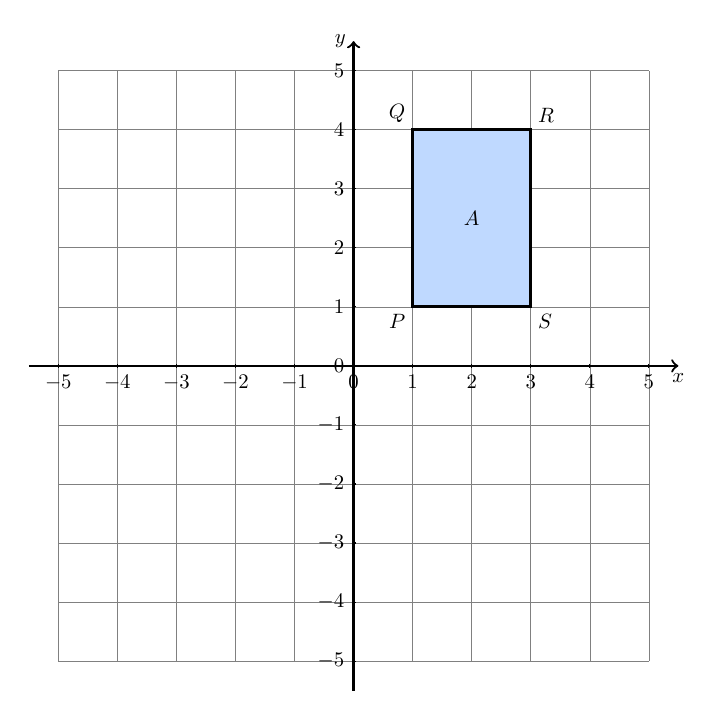
\begin{tikzpicture}[scale=0.75, transform shape]
    \definecolor{borderColour}{HTML}{000000}
    \definecolor{fillColourA}{HTML}{BFD9FF}

    \def\axisLimit{5}

    % Draw grid
    \draw[step=1cm,gray,very thin] (-\axisLimit,-\axisLimit) grid (\axisLimit,\axisLimit);

    % Draw axes
    \draw[thick,->] (-\axisLimit-0.5,0) -- (\axisLimit+0.5,0) node[anchor=north] {$x$};
    \draw[thick,->] (0,-\axisLimit-0.5) -- (0,\axisLimit+0.5) node[anchor=east] {$y$};

    % Label x-axis and y-axis
    \foreach \x in {-\axisLimit,...,\axisLimit}
        \draw (\x cm,1pt) -- (\x cm,-1pt) node[anchor=north] {$\x$};
    \foreach \y in {-\axisLimit,...,\axisLimit}
        \draw (1pt,\y cm) -- (-1pt,\y cm) node[anchor=east] {$\y$};

    % Shape A: vertices (1,1), (1,4), (3,4), (3,1)
    \coordinate (A1) at (1,1);
    \coordinate (A2) at (1,4);
    \coordinate (A3) at (3,4);
    \coordinate (A4) at (3,1);

    \filldraw[fill=fillColourA, draw=borderColour, line width=1pt] (A1) -- (A2) -- (A3) -- (A4) -- cycle;

    \node[below left] at (A1) {$P$};
    \node[above left] at (A2) {$Q$};
    \node[above right] at (A3) {$R$};
    \node[below right] at (A4) {$S$};
    \node at (2,2.5) {$A$};

\end{tikzpicture}
\end{center}

\noindent On a copy of the grid, reflect shape $A$ in the $x$-axis. Label the image $B$.

\vspace{4cm}

\begin{flushright}
    \answerlines{2}{2}
\end{flushright}
\end{question}